\chapter{BioBackgroundModels.jl: Parallel optimization of Hidden Markov Model zoos of genomic background noise}
\chaptermark{BBM.jl: Parallel optimization of background HMMs}
\label{chap:BBM}

\path{BioBackgroundModels.jl} (\path{BBM.jl} hereafter) is a pure Julia package intended to automate the optimization and selection of large numbers ("zoos") of Hidden Markov Models (HMMs), using sequence sampled from specified partitions of a given genome, on arbitrary collections of hardware. It is supplied with extensive utility functions for genomic sampling, high performance implementations of both the Baum-Welch and Churbanov-Winters algorithms for optimization of HMMs by expectation maximization (EM), as well as reporting functions for summarizing the results of the optimized model zoos. These tasks are necessary to select of models of genomic background noise, from which motif signals may be detected using a package such as \path{BioMotifInference.jl}.

HMMs generated by \path{BBM.jl} are standard $\geq$ 1 state HMMs that emit symbols corresponding to stretches of 1 or more base pairs. Following Down et al. \cite{Down2005}, the number of bases encoded by an HMM symbol is denoted by the ``order'' of the HMM. 0th order HMM emit 4 symbols, one for each of the genomic nucleotides, while 1\textsuperscript{st} order HMMs emit 16 symbols, one for each 2-base combination, and 2\textsuperscript{nd} order HMMs emit 64 symbols, one for each 3-base combination, and so on. It is expected that users will be interested in comparing the explanatory value of a variety of background HMM state numbers and orders in selecting appropriate background models. These can all be optimized in one batch; because high state and, to a lesser extent, high order numbers impose much more significant memory costs, the use of the Churbanov-Winters linear memory algorithm is strongly recommended\footnote{While the theoretical performance of the Churbanov-Winters algorithm is lower than Baum-Welch \cite{Churbanov2008}, the implementation herein is highly optimized and performant. For many use cases, it is both less memory-intensive and faster than Baum-Welch.}. A basic load balancing system has been provided to allow users to prefer particular machines for some optimization jobs over others, which permits the efficient use of clusters of dissimilar hardware in the batch context.

\section{Genome partitioning and sampling}
The optimization of an HMM zoo is performed against a sample of a ``genome partition'', which defines a portion of a genome in relation to a genomic feature set. The required files to sample from a genome partition are:

\begin{itemize}
    \item A whole-genome sequence in valid FASTA format (eg. a .fna or other appropriate nucleotide sequence file).
    \item An index for the genomic sequence file (eg. an .fna.fai file)
    \item A genomic feature file, annotating the genomic sequence, in GFF3 format
\end{itemize}

At present, \path{BBM.jl} offers a default strategy of sampling without replacement from exonic, periexonic, and intergenic partitions of genomes. This partition scheme is intended to differentiate between genomic sequences that are likely to differ in terms of the appropriateness of HMMs of different orders as background models. That is, the selective pressure imposed on genomic sequence by the codon code (exonic partition) and other higher-order functional features of gene organization (periexonic partition) are likely to favour different sorts of background HMM model than the simpler repetitive structure of intergenic material.

Sampling functions should normally be accessed through the API provided to the user. Firstly, sampling jobs may be set up by using the \path{setup_sample_jobs} function, which uses user-supplied paths to the files listed above, as well as user-specified partitioning variables, to divide the supplied genome into the partitions described and set up channels for these sampling jobs. For example:

\begin{minted}[breaklines,
               mathescape,
               linenos,
               numbersep=5pt,
               frame=lines,
               framesep=2mm]{julia}
using BioBackgroundModels
#FILE PATHS
danio_gff_path = "Danio_rerio.GRCz11.94.gff3"
danio_genome_path = "GCA_000002035.4_GRCz11_genomic.fna"
danio_gen_index_path = "GCA_000002035.4_GRCz11_genomic.fna.fai"

#CONSTANTS FOR GENOMIC SAMPLING
const sample_set_length = Int64(4e6)
const sample_window_min = 10
const sample_window_max = 3000
const perigenic_pad = 500

channels = setup_sample_jobs(danio_genome_path, danio_gen_index_path, danio_gff_path, sample_set_length, sample_window_min, sample_window_max, perigenic_pad)
\end{minted}

Here, \path{sample_set_length} defines the overall number of bases to be sampled from each partition, while \path{sample_window_min} and \path{sample_window_max} define the minimum and maximum length of each individual sample to be taken, without replacement, from the partitions. \path{sample_set_length} should be chosen to supply both training and test sets for background model selection; ie. it should be twice the desired length of the observation set in training. Lastly, \path{perigenic_pad} defines the number of bases up- and down-stream of the first and last codon to consider, along with intronic material, as constituting the ``perigenic'' partition. This will include promoter elements, splicing signals, and the like.

Secondly, the partitions are sampled (in parallel, by worker, if desired), to produce dataframes of samples and relevant coordinate and strand orientation information:

\begin{minted}[breaklines,
    mathescape,
    linenos,
    numbersep=5pt,
    frame=lines,
    framesep=2mm]{julia}
using Distributed,Serialization
sample_output = "samples"
worker_pool = addprocs(3)
sample_record_dfs=execute_sample_jobs(channels, worker_pool)
serialize(sample_output, sample_record_dfs)
\end{minted}

Here, one worker per partition is used to sample; lower numbers of workers will also work while larger numbers are of no benefit. In this example, the sample dataframes are serialized to the file ``samples'' for later use; they can also be used directly as described below.

\section{Optimizing BHMMs by EM algorithms}
Background HMM optimization by the expectation-maximization algorithms is performed by a similar two-step setup-and-execute functional pattern as genome sampling. Firstly, \path{setup_EM_jobs!} is used to transform supplied ``job IDs'' and the observations supplied by genome sampling into sets of EM chains to be elongated by the EM algorithm. \path{BBM.jl} ``job IDs'' take the form of \path{Chain_ID} structs, whose fields specify a string denoting the partition that forms the observations for the optimization, the number of states in the HMM, the order of the HMM's emitted symbols, and an integer denoting the replicate number of the chain. In general, for any given partition, number of states, and emission order, three or more replicates are advised, to confirm that the converged values of any particular HMM are likely to be near the global optimum \cite{Yang2015b}. That is, if replicates of some job ID chain all terminate with similar parameter values (see \autoref{sec:BBMdisplay} to examine this using \path{BBM.jl}), one such chain may reasonably be selected as a representative of the likely global optimum present in this region of the parameter space.

The helper function \path{split_obs_sets} is used to divide the genomic sample dataframes generated by the sampling API, described above, into training and test sets for optimization. The training set is supplied for the use of the EM algorithms, while the test set is used solely to calculate the final likelihoods of optimized models.

By default, \path{BBM.jl} initialises new HMM chains by sampling randomly from possible emission vectors, with strong priors on transition matrices with robust autotransition. Generally speaking, this tends to prevent chains from being optimized to trivial local minima with very short state residency times. This reflects our exclusive interest in those HMMs whose states represent stretches of nucleotides with shared biological significance; HMMs which tend to have state residency emission lengths of less than a few bases are of questionable biological relevance. If desired, the user may supply their own initialisation function as the \path{setup_EM_jobs!} keyword argument \path{init_function}, which defaults to \path{autotransition_init}. The default function should serve as the template for such user-defined initialisation functions.

\path{BBM.jl} operation is designed to be robust to most kinds of interruption, and the \path{setup_EM_jobs!} function may be used safely on existing sets of EM chains generated by BBM. This allows for resumption from interruption, reconfiguration of hardware, decreasing the desired chain termination threshold, and so on. The dict containing existing serialized chains, if any, should be supplied to the setup function as the \path{chains} keyword variable to allow this.

\begin{minted}[breaklines,
    mathescape,
    linenos,
    numbersep=5pt,
    frame=lines,
    framesep=2mm]{julia}
using BioBackgroundModels, DataFrames, Distributed, Serialization

#FILE PATHS
hmm_output = "chains"
sample_output = "samples"

#JOB CONSTANTS
const replicates = 3 #repeat optimisation from this many seperately initialised samples from the prior
const Ks = [1,2,4,6] #state #s to test
const order_nos = [0,1,2] #DNA kmer order #s to test
const delta_thresh=1e-5 #stopping/convergence criterion (log probability difference btw subsequent EM iterates)
const max_iterates=50000

#PROGRAMATICALLY GENERATE Chain_ID Vector
job_ids=Vector{Chain_ID}()
for (obs_id, obs) in training_sets, K in Ks, order in order_nos, rep in 1:replicates
    push!(job_ids, Chain_ID(obs_id, K, order, rep))
end

#SPLIT GENOME SAMPLES INTO TRAINING AND TEST SETS
sample_dfs = deserialize(sample_output)
training_sets, test_sets = split_obs_sets(sample_dfs)

#INTIIALIZE HMMS
if isfile(hmm_output) #if some results have already been collected, load them
    hmm_results_dict = deserialize(hmm_output)
else #otherwise, pass a new results dict
    hmm_results_dict = Dict{Chain_ID,Vector{EM_step}}()
end

em_jobset = setup_EM_jobs!(job_ids, training_sets; delta_thresh=delta_thresh, chains=hmm_results_dict)
\end{minted}

Once the EM jobset is set up, it is splatted into the \path{execute_EM_jobs!} function with any valid worker pool and the path for the Dict of EM chains to be serialized. All workers in the pool should be in \path{:master_worker} topology with the master process. \path{BBM.jl} workers will obtain new chains to elongate by EM until no more are available; the number of jobs, therefore, defines the useful upper limit for the number of workers in the pool.

Load balancing is achieved by using \path{BBM.jl}'s LoadConfig struct, whose fields define acceptable ranges of states, orders, and optional vectors of blacklisted and whitelisted \path{Chain_IDs}. A Dict of LoadConfigs keyed by Integer defines the appropriate LoadConfig to use for any given worker's integer id (ie. the output of \path{Distributed.myid()}).

The results of EM optimizations are serialized as they are ``pulled off the wire'', so that they cannot be lost by the algorithm being interrupted, network failure etc. Consequently, \path{execute_EM_jobs!} does not return anything that needs to be serialized for subsequent analyses; results are always located at the path provided to the function and may be freely inspected by the tools described in \autoref{sec:BBMdisplay} at any time during or after the optimization.

An example of \path{execute_EM_jobs!} usage, following from the setup example given above:

\begin{minted}[breaklines,
    mathescape,
    linenos,
    numbersep=5pt,
    frame=lines,
    framesep=2mm]{julia}
#SETUP LOAD BALANCING
local_config=LoadConfig(1:6,0:2)
remote_config=LoadConfig(1:4,0:1)

load_dict=Dict{Int64,LoadConfig}()

worker_pool=addprocs(no_local_processes, topology=:master_worker)
for worker in worker_pool
    load_dict[worker]=local_config
end

remote_pool=addprocs([(remote_machine,no_remote_processes)], tunnel=true, topology=:master_worker)

for worker in remote_pool
    load_dict[worker]=remote_config
end

worker_pool=vcat(worker_pool, remote_pool)

#EXECUTE EM JOBS
execute_EM_jobs!(worker_pool, em_jobset..., hmm_output; load_dict=load_dict, delta_thresh=delta_thresh, max_iterates=max_iterates)
\end{minted}

\section{BHMM analysis and display}
\label{sec:BBMdisplay}
A report generation and display API is provided in order to analyse the results of optimizing a zoo of background HMMs using \path{BBM.jl}. One function, \path{generate_reports}, serves to prepare all of the available reports on the zoo. Its use is straightforward:

\begin{minted}[breaklines,
    mathescape,
    linenos,
    numbersep=5pt,
    frame=lines,
    framesep=2mm]{julia}
chains=deserialize(hmm_output)
sample_dfs = deserialize(sample_output)
training_sets, test_sets = split_obs_sets(sample_dfs)

report_folders=generate_reports(chains, test_sets)
serialize(survey_folders, report_folders) #save reports
\end{minted}

\path{generate_reports} creates a Dict of \path{Report_Folder}s, keyed by partition id string. Each \path{Report_Folder} contains a \path{Partition_Report} with information about all HMMs trained on that partition, a \path{Replicate_Report} which enables the comparison of the replicates of the best model available for the partition, and a Dict of \path{Chain_Report}s keyed by \path{Chain_ID}, which give specific information concerning each chain produced for the partition. Examples of report output follow, derived from the model zoo training task whose results are summarised \autoref{BHMMlh}. The contents of the reports on background models trained on the \textit{D. rerio} ``exonic'' partition follow.

\begin{figure}[!h]
    \makebox[\textwidth][c]{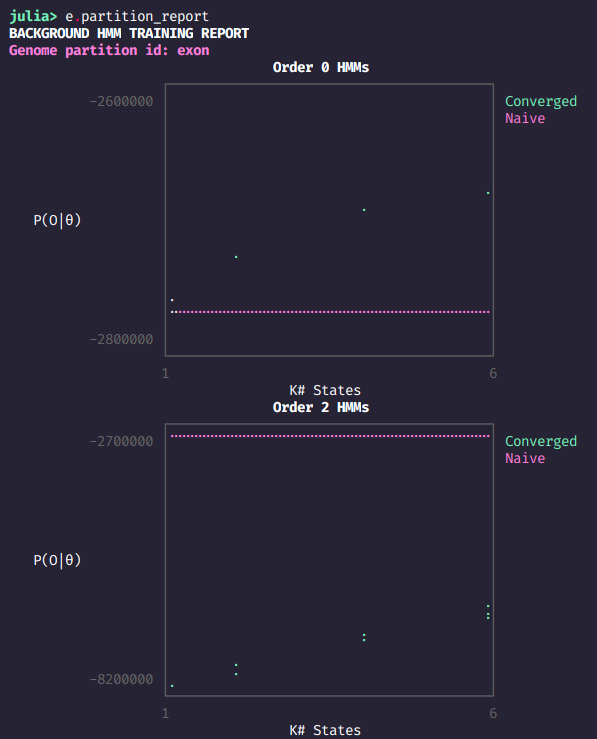
\includegraphics{BBM/partition_report.png}}    
    \caption{{\bf Example \protect\path{BBM.jl} Partition Report}}
    \label{partreport}
\end{figure}

\autoref{partreport} displays partial output from the \path{Partition_Report} associated with BHMM training on the exonic partition. The report identifies the partition in question, and, for each order of BHMM trained on the partition, displays a plot of the likelihood of the models vs. the number of states in the model. In this case, 0\textsuperscript{th} and 2\textsuperscript{nd} order models are displayed. The likelihood of a naive, 0\textsuperscript{th}-order, 1-state model with equal emission probability for each symbol serves as a benchmark for BHMM likelihood; this value is plotted as a magenta line across the state axis. In this case, all 0\textsuperscript{th}-order models are more likely descriptions of \textit{D. rerio} exonic material than a naive model, while all 2\textsuperscript{nd}-order models fall below this benchmark likelihood. This reflects the greatly expanded parameter space associated with 64 emission symbols. Thus, the additional exonic order capturable by 3mers is insufficient to offset the decreased probability of any given sequence using this many symbols.

Individual models are plotted as scatterplot points. Converged models are rendered in green, unconverged models in red\footnote{The reports API is agnostic about the state of the model zoo reported on; it can be used to monitor zoos before they are fully converged.}. In this case, no unconverged models are present. The 0\textsuperscript{th}-order models are tightly converged such that their likelihoods are not differentiable, while the 2\textsuperscript{nd}-order models are more spread out across the larger parameter space. The intended use of this report is to perform a quick visual assessment of the state of the zoo trained on the specified partition, before proceeding to the \path{Replicate_Report} and particular \path{Chain_Report}s.

\begin{figure}[!h]
    \makebox[\textwidth][c]{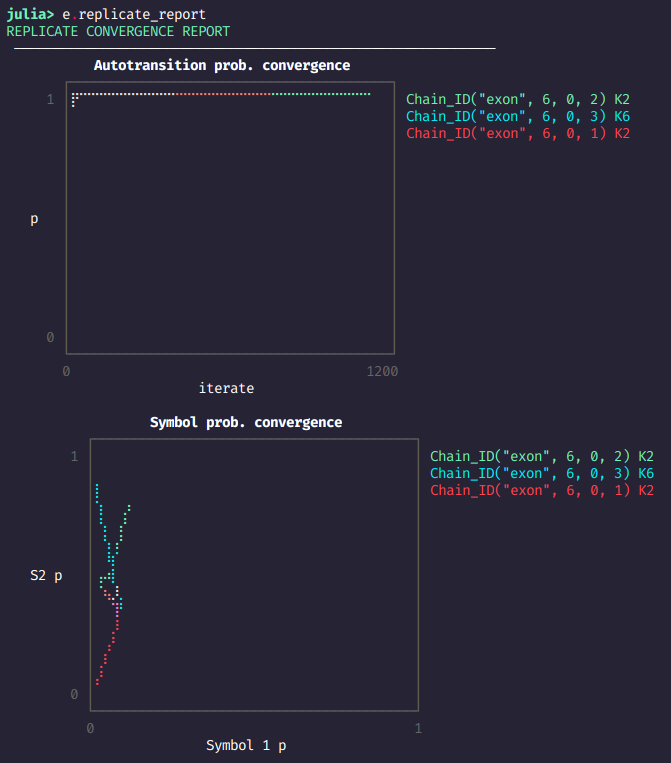
\includegraphics{BBM/replicate_report.png}}    
    \caption{{\bf Example \protect\path{BBM.jl} Replicate Report}}
    \label{repreport}
\end{figure}

\autoref{repreport} displays partial output from the exonic \path{Replicate_Report}. The chains displayed in the report are the most likely replicate set for the partition. The report consists of paired convergence plots for the autotransition probabilities and 2-dimensional symbol emission probabilities for each state and each replicate in the set. Because there is no guarantee that HMMs from th same optima will have the same ordering of states, similar states are identified by minimizing the Euclidean distance between state emission vectors across the trained replicates. In this case, replicate 1's second state (red) is also identified with the second state of replicate 2 (green), but the sixth state of replicate 3 (blue).

The autotransition probability subplot displays the transition matrix diagonal probability for the designated state and replicates (that is, the probability that the HMM will stay in the state). If the HMMs are correctly converged on a global optimum, the autotransition probabilities for all chains should terminate at nearly the same value. Given that this probability will be stationary on converged chains, this can be visually confirmed by looking for substantial horizontal overlap of the chain autotransition probabilities for the state, as seen in \autoref{repreport}.

The symbol probability subplot displays the evolution of the probability of the first symbol emitted by the state plotted against the probability of the second symbol, providing a simple two-dimensional view into the convergence of the state's emission vector. If the chains are correctly converged on the global optimum, the plot's appearance should show chains from divergent areas of this two-dimensional parameter subset converging on the same values for the two symbols, as seen in \autoref{repreport}.

\path{Chain_Report}s for all HMMs trained on the partition are available in a Dict keyed by \path{Chain_ID}, found at the \path{chain_reports} field of the report folder. Example output for replicate 1 from the above-described replicate set is presented below. \path{Chain_Report}s consist of three major sections, described in turn.

\begin{figure}[!h]
    \makebox[\textwidth][c]{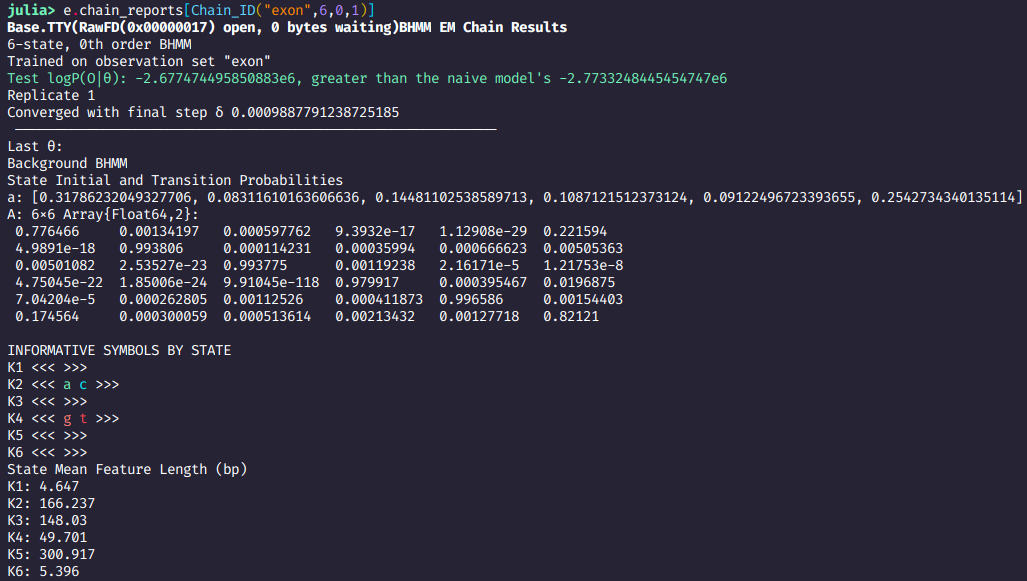
\includegraphics{BBM/chain_report1.png}}    
    \caption{{\bf Example \protect\path{BBM.jl} Chain Report - Part 1}}
    \label{chreport1}
\end{figure}

The first \path{Chain_Report} section begins by stating the state number and order of the BHMM, as well as the genomic partition on which it was trained. This is followed by the likelihood of the model given the test observation set, compared to the naive model. The line stating these likelihoods will be green if the BHMM is better than the naive model, red if not. The general information concludes with the replicate number of the BHMM, as well as the convergence status of the chain and the final EM step size.

The section continues by stating the initial state probability vector $a$ and the state transition matrix $A$ for the converged BHMM. Emission vectors for the BHMMs' state are summarized by their informational content; symbols with $\geq$ .7 bits of information are printed in bold capital characters, those with .7 $\>$ information $\geq$ .25 are printed in capital characters, those with .25 $\>$ information $\geq$ .05 are printed with lowercase characters, and those with less than .05 bits are not printed at all. In this case, state 2 emits adenine and cytosine symbols more frequently than guanine or thymidine, while this is reversed in state 4. The other states have similar enough emission probabilities for the four bases that they do not register on the informative symbols display. This gives a rough idea of what sort of information the BHMM states encode.

The last part of this section presents an estimate of the mean feature length for each state, meaning the mean number of bases emitted from the state before transitioning to a new state (otherwise known as ``state residency time'' and similar concepts). This is estimated by \hyperref[ssec:MonteCarlo]{Monte Carlo} sampling of run lengths, given the autotransition probabilities for the BHMM. This is intended to give an idea of the biological relevance of the sequence features emitted by the BHMM's states. Generally speaking, most ``background noise'' features, like intergenic CpG islands, are held to be on the order of hundreds of bases. Users should expect good BHMMs to have some states that tend to emit features around this size.

\begin{figure}[!h]
    \makebox[\textwidth][c]{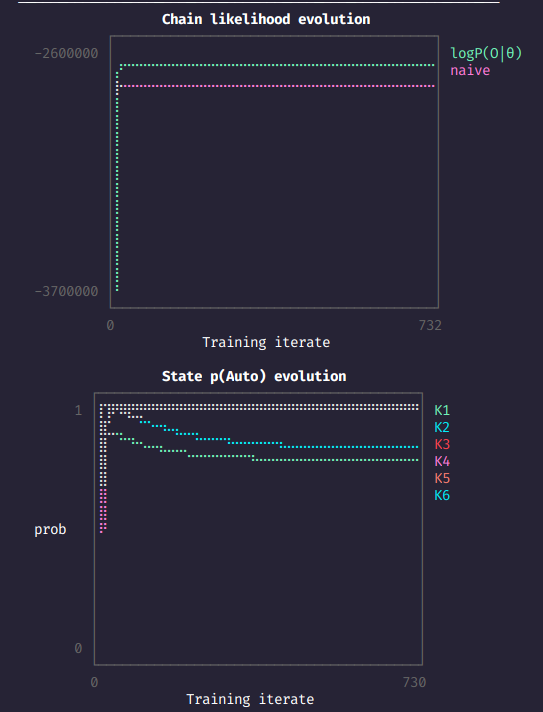
\includegraphics{BBM/chain_report2.png}}    
    \caption{{\bf Example \protect\path{BBM.jl} Chain Report - Part 2}}
    \label{chreport2}
\end{figure}

The second part of the \path{Chain_Report}, displayed in \autoref{chreport2}, displays the evolution of the model's likelihood and state autotransition probabilities over the chain iterates. This is primarily intended as a visual aid to the convergence tests presented in the third part of the report. Both the model likelihood and autotransition probabilities should be stationary over the last portion of the chain for it to be considered legitimately converged. This can be numerically confirmed in the third part of the report.

\begin{figure}[!h]
    \makebox[\textwidth][c]{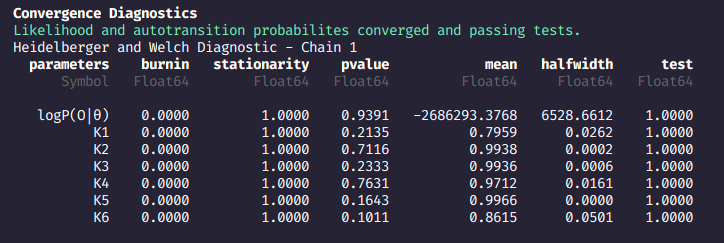
\includegraphics{BBM/chain_report3.png}}    
    \caption{{\bf Example \protect\path{BBM.jl} Chain Report - Part 3}}
    \label{chreport3}
\end{figure}

The third part of the \path{Chain_Report} displays the output of the Heidelberger and Welch convergence diagnostic \cite{Heidelberger1981}, as implemented by \path{MCMCChains.jl} \cite{Pfiffer2020}. Both the BHMM likelihood and the autotransition probability for each state are tested for stationarity. A chain from a good replicate set (as assessed by the \path{Replicate_Report}) that passes these diagnostic tests is reasonably considered properly converged on the global optimum for the partition samples used as the training set. If this is so, a green test-passing statement will be printed, if not, a red failure statement. The specific reason for failure can be determined by finding the parameters with a test value of 0. Taken together, these reports can be used to verify that the EM optimization is functioning properly, and that appropriately converged models are chosen to represent genomic background noise from the partition of interest.

\section{Numerical accuracy and tests}
Because \path{BBM.jl} contains two different \hyperref[ssec:EM]{EM} algorithms, these are used internally to check for numerical accuracy and consistency. In general, input to either Baum-Welch or Churbanov algorithms should produce nearly-identical output (i.e. isapprox() will return true). Additionally, some lower-performance implementations are available under \path{BBM.jl/src/test/ref_fns.jl} for comparison. A fairly comprehensive test suite is provided, and can be executed using \path{]test BioBackgroundModels}. So long as tests are passing, numerical accuracy of the EM algorithms is established. The tests make use of a synthetic FASTA-format genome to test the genome sampling routines. Passing tests indicates that this system is working as intended. 

\section{Future directions}

\path{BBM.jl} is largely feature complete. However, the genomic sampling regime implemented for this thesis is unnecessarily restrictive. In particular, there is no provision for common tasks like assembling the upstream promoter sequences of some group of genes with a common functional annotation. This could be improved by implementing a partition definition system that uses user-defined feature- and coordinate-based masking of the genome to assemble custom partitions. This would make \path{BBM.jl} a useful generalist tool for establishing background models when inferring genomic signals.